\documentclass[aspectratio=169]{beamer}

\usetheme{CambridgeUS}
\usecolortheme{default} % red color scheme standard CambridgeUS

\usepackage{amsmath, amssymb}
\usepackage{graphicx}
\usepackage{subcaption}
\usepackage{booktabs}
\usepackage{xcolor}
\usepackage{tikz}

\usepackage{dirtree}
\usepackage{lmodern}
\usepackage{microtype}

% Colori per le categorie
\definecolor{colMain}{RGB}{0,70,140}
\definecolor{colAssembly}{RGB}{180,60,0}
\definecolor{colMesh}{RGB}{0,120,60}
\definecolor{colPost}{RGB}{120,0,120}
\definecolor{colTools}{RGB}{100,80,0}
\definecolor{colError}{RGB}{160,0,40}
 
\newcommand{\cmt}[2]{{\footnotesize\texttt{#1}\enspace{\color{gray!80!black}--- #2}}}
% -------------------------------------------------------
% Title info
% -------------------------------------------------------
\title[FEM/BEM Coupling]{Coupled FEM/BEM:\\
  Open-Domain Conditions in 2D Electrostatics}
\subtitle{Computational Electromagnetics}
\author[Matteo Morana]{Matteo Morana}
\institute[PoliMi]{Master in Mathematical Engineering\\
  Politecnico di Milano}
\date{April 28, 2026}

% -------------------------------------------------------
\begin{document}

\begin{frame}
  \titlepage
\end{frame}

% -------------------------------------------------------
% \begin{frame}{Outline}
%   \tableofcontents
% \end{frame}

% ===============================================================
\section{Motivation}
% ===============================================================

\begin{frame}{The Problem: Parallel-Plate Capacitor in 2D}

  \begin{columns}
    \begin{column}{0.55\textwidth}
      Solve Laplace's equation in the whole plane:
      \[
        \Delta u = 0 \quad \text{in } \mathbb{R}^2 \setminus \{\text{plates}\}
      \]
      with Dirichlet conditions on the plates:
      \[
        u = +V \;\text{(top)}, \qquad u = -V \;\text{(bottom)}
      \]

      \bigskip
      \textbf{Goal:} compute the electric potential \emph{both inside and outside}
      the capacitor in a real case scenario.
    \end{column}
    \begin{column}{0.42\textwidth}
      \centering
      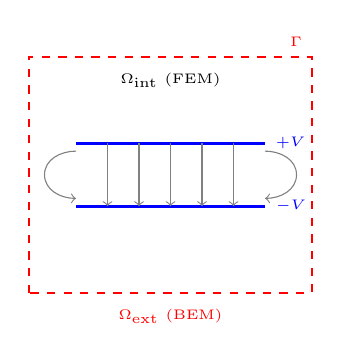
\begin{tikzpicture}[scale=1.0]
        % Outer box
        \draw[dashed, red, thick] (-1.8,-1.5) rectangle (1.8,1.5)
          node[above left, red, font=\tiny] {$\Gamma$};
        % Plates
        \draw[very thick, blue] (-1.2, 0.4) -- (1.2, 0.4)
          node[right, font=\tiny] {$+V$};
        \draw[very thick, blue] (-1.2,-0.4) -- (1.2,-0.4)
          node[right, font=\tiny] {$-V$};
        % Field lines sketch
        \foreach \x in {-0.8,-0.4,0.0,0.4,0.8}{
          \draw[->, gray, thin] (\x, 0.4) -- (\x, -0.4);
        }
        % Fringing
        \draw[->, gray, thin] (1.2, 0.3) to[out=0,in=90] (1.6, 0.0)
          to[out=-90,in=0] (1.2,-0.3);
        \draw[->, gray, thin] (-1.2, 0.3) to[out=180,in=90] (-1.6, 0.0)
          to[out=-90,in=180] (-1.2,-0.3);
        % Labels
        \node[font=\tiny] at (0, 1.2) {$\Omega_{\text{int}}$ (FEM)};
        \node[font=\tiny, red] at (0,-1.8) {$\Omega_{\text{ext}}$ (BEM)};
      \end{tikzpicture}
    \end{column}
  \end{columns}

\end{frame}

% -------------------------------------------------------
\begin{frame}{Why Not Pure FEM?}

  \begin{block}{Pure FEM approach}
    Truncate the domain; impose $u=0$ on the artificial boundary $\Gamma$.
  \end{block}

  \medskip
  \textbf{Drawbacks:}
  \begin{itemize}
    \item Requires a \textbf{very large domain} to minimize the truncation error
          ($\Gamma$ must be placed at $\sim 50\,L_y$ from the plates).
    \item Leads to \textbf{large meshes} and long computation times.
    \item Cannot represent the solution \textbf{up to infinity}: introduces an
          unavoidable approximation.
  \end{itemize}

  \medskip
  \begin{alertblock}{Key idea}
    Use \textbf{FEM} inside a small domain and \textbf{BEM} to handle the
    exterior exactly — including infinity.
  \end{alertblock}

\end{frame}

% ===============================================================
\section{FEM Formulation}
% ===============================================================

\begin{frame}{FEM Weak Formulation}

  Starting from the Laplace problem on a bounded domain $\Omega$:
  \[
    \Delta u = 0 \quad \Longrightarrow \quad
    \int_\Omega \nabla u \cdot \nabla v\,dx
    - \underbrace{\int_{\partial\Omega} \frac{\partial u}{\partial n} v\,ds}_{\text{boundary term}}
    = 0 \qquad \forall v \in H^1(\Omega)
  \]

  \medskip
  After discretisation with basis $\{v_i\}_{i=1}^{N_h}$, writing
  $u \approx \sum_j u_j v_j$ and
  $\dfrac{\partial u}{\partial n} \approx \sum_j \dfrac{\partial u_j}{\partial n} v_j$:

  \[
    \textcolor{green!60!black}{S}\,\textcolor{blue}{\mathbf{u}}
    \;-\;
    \textcolor{green!60!black}{T}\,\textcolor{red}{\dfrac{\partial\mathbf{u}}{\partial n}}
    = \mathbf{0}
  \]

  where $S_{ij} = \displaystyle\int_\Omega \nabla v_i\cdot\nabla v_j\,dx$
  and $T_{ij} = \displaystyle\int_{\partial\Omega} v_i\,v_j\,ds$.

\end{frame}

% -------------------------------------------------------
\begin{frame}{Variable Count — The Key Issue}

  \begin{block}{How many unknowns?}
    The system provides $N_h$ equations. The unknowns are:
    \begin{itemize}
      \item $\textcolor{blue}{u_j}$, $j=1,\ldots,N_h$ \quad nodal potential values
      \item $\textcolor{red}{\partial u_j/\partial n}$, $j=1,\ldots,N_h$ \quad
            normal-derivative coefficients
    \end{itemize}
    \[
      N_h \text{ equations} \quad \text{vs} \quad 2N_h \text{ unknowns}
      \quad \Rightarrow \quad \text{\textbf{under-determined!}}
    \]
  \end{block}

  \medskip
  \textbf{Rescue: Lagrange nodal basis functions} satisfy $v_i(x_j)=\delta_{ij}$, so
  \[
    v_i\big|_{\partial\Omega} = 0 \quad \text{for every \emph{interior} node } i
    \quad\Longrightarrow\quad
    T_{ij} = 0 \text{ if } i \text{ or } j \text{ is interior.}
  \]

  \medskip
  \begin{alertblock}{Variable reduction}
    \begin{itemize}
      \item Normal-derivative unknowns at \emph{interior} nodes drop out of the system.
      \item System: $N_h$ equations, $N_h + N_h^\partial$ unknowns.
            Here BEM provide $N_h^\partial$ equations.
    \end{itemize}
  \end{alertblock}
\end{frame}

% -------------------------------------------------------
\begin{frame}{FEM Block Structure}

  Partitioning nodes into \textbf{interior} ($I$) and \textbf{boundary} ($B$):

  \[
    \underbrace{
    \begin{bmatrix}
      S_{II} & S_{IB} \\[4pt]
      S_{BI} & S_{BB}
    \end{bmatrix}
    }_{\text{FEM stiffness}}
    \begin{bmatrix} \textcolor{blue}{u_I} \\[4pt] \textcolor{blue}{u_B} \end{bmatrix}
    -
    \begin{bmatrix} \mathbf{0} \\[4pt] T_{BB}\,\textcolor{red}{\dfrac{\partial u_B}{\partial n}} \end{bmatrix}
    = \mathbf{0}
  \]

  \bigskip
  \begin{itemize}
    \item Row $I$: closed — $\partial u/\partial n$ does not appear.
    \item Row $B$: \textbf{open} — involves the unknown
          $\textcolor{red}{\partial u_B/\partial n}$ (will be supplied by BEM).
  \end{itemize}

\end{frame}

% ===============================================================
\section{BEM Formulation}
% ===============================================================

\begin{frame}{BEM — Boundary Integral Equation}

  \textbf{Key idea:} reformulate the Laplace problem on $\partial\Omega$ only,
  using the fundamental solution $G(x,y) = \frac{1}{2\pi}\log|x-y|$ in 2D.

  \bigskip
  Green's third identity $\Rightarrow$ \textbf{Boundary Integral Equation} (BIE):
  \[
    \frac{1}{2}\,u(y) = \underbrace{\int_{\partial\Omega} G(x,y)\,
    \frac{\partial u}{\partial n}(x)\,ds_x}_{\mathcal{V}(\partial u/\partial n)(y)}
    \;-\;
    \underbrace{\int_{\partial\Omega} \frac{\partial G}{\partial n_x}(x,y)\,u(x)\,ds_x}_{
      \mathcal{K}(u)(y)}
    \qquad \forall\, y \in \partial\Omega
  \]

  \bigskip
  After collocation discretizations with boundary basis $\{\psi_j\}$:
  \[
    H\,\textcolor{blue}{u_B} = G\,\textcolor{red}{\dfrac{\partial u_B}{\partial n}}
    \qquad
    H = \tfrac{1}{2}M + K, \quad G \text{ symmetric}
  \]

  \begin{block}{}
    BEM provides \textbf{exactly} $N_h^\partial$ equations relating $u_B$ and
    $\partial u_B/\partial n$ — the missing relations from FEM.
  \end{block}

\end{frame}

% ===============================================================
\section{FEM-BEM Coupling}
% ===============================================================
\begin{frame}{Coupled System and Plates Conditions}
  Replace the open FEM boundary rows with the BEM equations:
  \[
    \begin{bmatrix}
      S_{FF} & S_{FD} & S_{FB} \\[4pt]
      S_{DF} & S_{DD} & S_{DB} \\[4pt]
      S_{BF} & S_{BD} & S_{BB}
    \end{bmatrix}
    \begin{bmatrix}
      \textcolor{blue}{u_F} \\[4pt]
      \textcolor{blue}{u_D} \\[4pt]
      \textcolor{blue}{u_B}
    \end{bmatrix}
    -
    \begin{bmatrix}
      0 \\[4pt] 0 \\[4pt] -T_{BB}\,\textcolor{red}{\dfrac{\partial u_B}{\partial n}}
    \end{bmatrix}
    =
    \begin{bmatrix} \mathbf{0} \\ \mathbf{0} \\ \mathbf{0} \end{bmatrix}
  \]
  \medskip
  \begin{itemize}
    \item \textbf{Row 1 (FEM, free):} governs $u$ at unconstrained interior nodes.
    \item \textbf{Row 2 (FEM, Dirichlet):} enforces the prescribed potential on the plates.
    \item \textbf{Row 3 (FEM--BEM, boundary):} couples the FEM domain to the exterior via $T_{BB}\,G^{-1}H$.
  \end{itemize}
\end{frame}

% -------------------------------------------------------
\begin{frame}{Elimination and Reduced System}

  Assume $G$ invertible:
  \[
    \frac{\partial u_B}{\partial n} = -G^{-1}H\,u_B
  \]

  Substitute into the FEM boundary row $\Rightarrow$ \textbf{reduced system of size $N_h$}:

  \[
    \begin{bmatrix}
      S_{II} & S_{IB} \\[4pt]
      S_{BI} & S_{BB} + \underbrace{T_{BB}\,G^{-1}H}_{\text{BEM correction (dense)}}
    \end{bmatrix}
    \begin{bmatrix} u_I \\[4pt] u_B \end{bmatrix}
    =
    -\begin{bmatrix} S_{ID} \\ S_{BD} \end{bmatrix} u_D
  \]

  \begin{itemize}
    \item Same size as a standard FEM system ($N_h \times N_h$).
    \item The BEM term $T_{BB}G^{-1}H$ is \textbf{dense} but restricted to boundary DOFs.
    \item In MATLAB: $G^{-1}H$ computed via the backslash operator.
    \item After solving: recover $\partial u_B/\partial n$ and the exterior potential via
          the BEM representation formula.
  \end{itemize}

\end{frame}

% ===============================================================
\section{Comparison with Pure FEM}
% ===============================================================

\begin{frame}{Setup}

  \begin{columns}
    \begin{column}{0.55\textwidth}
      \textbf{Geometry:}
      \begin{itemize}
        \item $L_x = 0.05$ m, $L_y = 0.05$ m ($L_x/L_y = 1$)
        \item $V_1 = 0.5$ V (top), $V_2 = -0.5$ V (bottom)
        \item $\Gamma$ placed at $3\,L_y$ margin on all sides
        \item $\varepsilon_r = 1$
      \end{itemize}
      \textbf{Meshes:}
      \begin{itemize}
        \item Coarse: $\delta = 0.005$ m $\approx 5000$ nodes
      \end{itemize}
      \textbf{Reference:} 
      \paragraph{The reference is a pure FEM method with a Dirichlet condition imposed on $\Gamma$ placed at $50L_y$}
    \end{column}
    \begin{column}{0.42\textwidth}
    \centering
    \resizebox{0.70\linewidth}{!}{%
      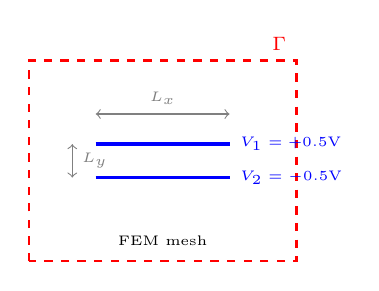
\begin{tikzpicture}[scale=0.85]
        % Dominio
        \draw[red, dashed, thick] (0,0) rectangle (4,3)
          node[above left, red, font=\scriptsize]{$\Gamma$};
    
        % Piastre
        \draw[very thick, blue] (1,1.75)--(3,1.75)
          node[right, font=\tiny]{$V_1=+0.5$V};
        \draw[very thick, blue] (1,1.25)--(3,1.25)
          node[right, font=\tiny]{$V_2=-0.5$V};
    
        % Indicatore Lx
        \draw[<->,gray] (1,2.2)--(3,2.2)
          node[midway,above,font=\tiny]{$L_x$};
    
        % Indicatore Ly
        \draw[<->,gray] (0.65,1.25)--(0.65,1.75)
          node[midway,right,font=\tiny]{$L_y$};
    
        % Mesh label
        \node[font=\tiny] at (2,0.3){FEM mesh};
      \end{tikzpicture}
    }%
    
    
\includegraphics[width=0.85\linewidth]{Documentation/runs/mesh_zoom.png}
    \end{column}
    \end{columns}
\end{frame}

% ===============================================================
    
\begin{frame}{FEM-BEM vs.\ Pure FEM}

  \begin{columns}
    \begin{column}{0.48\textwidth}
      \centering
      
\includegraphics[width=0.6\linewidth]{Documentation/runs/mesh_0050/margin_3/png/FEM_50_BEM_3.png}\\
      \small Pure FEM ($50\,L_y$ domain) — reference solution
    \end{column}
    \begin{column}{0.48\textwidth}
      \centering
      
\includegraphics[width=\linewidth]{Documentation/runs/mesh_0050/margin_3/png/u_err_FEM_50_BEM_3.png}\\
      \small Pointwise difference: FEM vs.\ FEM-BEM on common domain
    \end{column}
  \end{columns}

  \medskip
  \[
    \varepsilon_{L^2} =
    \sqrt{\frac{\sum_{i\in\mathcal{N}_c}(u_i^{\text{FEM}}-u_i^{\text{FEM-BEM}})^2}
               {\sum_{i\in\mathcal{N}_c}(u_i^{\text{FEM}})^2}}
    \times 100\% \;=\; \mathbf{3.44\%}
  \]

\end{frame}

% -------------------------------------------------------
\begin{frame}{FEM-BEM vs.\ Pure FEM — Accuracy \& Speed}

  \begin{columns}
    \begin{column}{0.48\textwidth}
      \centering
      
\includegraphics[width=\linewidth]{Documentation/runs/mesh_0050/margin_3/png/L2_norm.png}\\
      \small $L^2$ error vs.\ FEM domain size
    \end{column}
    \begin{column}{0.48\textwidth}
      \centering
      
\includegraphics[width=\linewidth]{Documentation/runs/mesh_0050/margin_3/png/time.png}\\
      \small Computational time comparison
    \end{column}
  \end{columns}

  \medskip
  \begin{block}{Efficiency gain \textit{on my computer}}
    \begin{itemize}
      \item FEM-BEM ($3\,L_y$ domain): \textbf{8.52 s}
      \item Pure FEM ($50\,L_y$ domain): \textbf{2800 s} ($\approx 47$ min)
    \end{itemize}
  \end{block}

\end{frame}

% ===============================================================

\section{Numerical Results - FEM-BEM}
% ===============================================================



% -------------------------------------------------------
\begin{frame}{Electric Potential Distribution FEM-BEM}

  \begin{columns}
    \begin{column}{0.48\textwidth}
      \centering
      
\includegraphics[width=\linewidth]{Documentation/runs/mesh_0050/margin_3/png/potential_map.png}\\
      \small Potential map ($\delta=0.005$ m)
    \end{column}
    \begin{column}{0.48\textwidth}
      \centering
      
\includegraphics[width=\linewidth]{Documentation/runs/mesh_0050/margin_3/png/potential_contour.png}\\
      \small Equipotential lines
    \end{column}
  \end{columns}

  \medskip
  \begin{itemize}
    \item Uniform field between plates; smooth fringing at edges.
  \end{itemize}

\end{frame}

% -------------------------------------------------------
\begin{frame}{Electric Field FEM-BEM}

  \begin{columns}
    \begin{column}{0.48\textwidth}
      \centering
      
\includegraphics[width=\linewidth]{Documentation/runs/mesh_0050/margin_3/png/Efield_map_zoom.png}\\
      \small $\delta = 0.005$ m (coarse)
    \end{column}
    \begin{column}{0.48\textwidth}
      \begin{itemize}
    \item Central field $\approx (V_1-V_2)/L_y = 20$ V/m as expected.
    \item Fine mesh resolves singularity at plate corners (physically expected).
    \item Coarse mesh smears the edge singularity.
  \end{itemize}
    \end{column}
  \end{columns}


\end{frame}

% -------------------------------------------------------
\begin{frame}{Electric Field — Element Analysis (FEM-BEM)}

  \begin{columns}
    \begin{column}{0.48\textwidth}
      \centering
      
\includegraphics[width=\linewidth]{Documentation/runs/mesh_0050/margin_3/png/Efield_bad_elements.png}\\
      \small Elements with $|\mathbf{E}|>21$ V/m
    \end{column}
    \begin{column}{0.48\textwidth}
      \centering
      
\includegraphics[width=\linewidth]{Documentation/runs/mesh_0050/margin_3/png/Efield_histogram.png}\\
      \small Distribution of $|\mathbf{E}|$ per element
    \end{column}
  \end{columns}

  \medskip
  \begin{itemize}
    \item Anomalous elements localised at plate \textbf{corners} only.
    \item This is a well-known physical singularity of infinitely thin conductors
          — \textbf{not} a numerical artefact.
    \item The majority of elements have $|\mathbf{E}| \approx 20$ V/m.
  \end{itemize}

\end{frame}

% -------------------------------------------------------
\begin{frame}{Flux Through $\Gamma$ (FEM-BEM)}

  \begin{columns}
    \begin{column}{0.48\textwidth}
      \centering
      
\includegraphics[width=\linewidth]{Documentation/runs/mesh_0050/margin_3/png/q_gamma.png}\\
      \small $\partial u/\partial n$ on $\Gamma$
    \end{column}
    \begin{column}{0.48\textwidth}
      \textbf{Physical expectation:}
      \begin{itemize}
        \item Net flux must vanish (equal and opposite plate charges).
      \end{itemize}
      \[
        Q_{tot} =\oint_\Gamma \frac{\partial u}{\partial n}\,ds \approx -1.79\times10^{-13} \approx 0
      \]
      \vspace{-0.5em}
      Numerically consistent with zero — coupling condition verified.
    \end{column}
  \end{columns}

\end{frame}

% -------------------------------------------------------
\begin{frame}{Surface Charge Density and Capacitance}

  \begin{columns}
    \begin{column}{0.50\textwidth}
      \centering
      
\includegraphics[width=\linewidth]{Documentation/runs/mesh_0050/margin_3/png/charge_density.png}\\
      \small Surface charge density on the plates
    \end{column}
    \begin{column}{0.35\textwidth}
\textbf{Charge method:}
    \[
    C = \frac{|Q|}{V_1 - V_2}
    \]
    \begin{itemize}
        \item $C_{\text{FEM-BEM}} = 9.9811 \times 10^{-12}$ F/m
        \item $C_{\text{FEM}} = 9.9824 \times 10^{-12}$ F/m
    \end{itemize}

    \end{column}
    
  \end{columns}

\end{frame}

% -------------------------------------------------------
\begin{frame}{Capacitance different Ly, fixed Lx}

  \begin{columns}
    \begin{column}{0.44\textwidth}
      \centering
      
\includegraphics[width=\linewidth]{Documentation/runs/mesh_0050/margin_10/comparison_capacitance.png}\\
      \small Capacitance with different Ly
    \end{column}
    \begin{column}{0.53\textwidth}
      \small

      \medskip
      \begin{itemize}
        \item \textbf{Method comparison:} internal energy method inside the capacitor shows excellent agreement; charge-based method slightly overestimates
        \item \textbf{Full domain energy:} increasing deviation from theory due to energy stored outside the capacitor
      \end{itemize}
    \end{column}
  \end{columns}

\end{frame}

% ===============================================================

\section{Conclusions \& Future Work}
% ===============================================================

\begin{frame}{Conclusions}

  \begin{itemize}
    \item A \textbf{FEM-BEM coupled solver} for 2D electrostatics has been implemented
          in MATLAB, targeting the parallel-plate capacitor problem.

    \item The coupling exploits:
      \begin{enumerate}
        \item FEM's accuracy in the bounded interior region.
        \item BEM's ability to represent the exterior field \textbf{up to infinity}.
      \end{enumerate}

    \item Validation confirms:
      \begin{itemize}
        \item Correct potential and field distributions.
        \item Capacitance within 0.69\% of the reference FEM solution.
        \item Gauss's law satisfied numerically.
      \end{itemize}

    \item \textbf{100$\times$ speed-up} over a comparable pure FEM simulation.
  \end{itemize}

\end{frame}


\begin{frame}{Simulation Parameters}

\begin{columns}[T]

% --- Left column ---
\begin{column}{0.48\textwidth}
  \textbf{\color{blue!70!black}Physical Domain}
  \vspace{0.3em}
  \begin{tabular}{@{}lp{4.2cm}@{}}
    \toprule
    \texttt{Lx}, \texttt{Ly} & Dimensions of the rectangular domain [m] \\
    \texttt{delx}, \texttt{dely} & Spatial discretization step (FEM grid) [m] \\
    \bottomrule
  \end{tabular}

  \vspace{0.8em}
  \textbf{\color{blue!70!black}Medium Properties}
  \vspace{0.3em}
  \begin{tabular}{@{}lp{4.2cm}@{}}
    \toprule
    \texttt{e0} & Permittivity of free space $\varepsilon_0 = 8.85\times10^{-12}$ F/m \\
    \texttt{er} & Relative permittivity of the medium $\varepsilon_r$ \\
    \bottomrule
  \end{tabular}
\end{column}

% --- Right column ---
\begin{column}{0.50\textwidth}
  \textbf{\color{blue!70!black}FEM--BEM Coupling}
  \vspace{0.3em}
  \begin{tabular}{@{}lp{4.2cm}@{}}
    \toprule
    \texttt{margin\_BEM\_coeff} & Coefficient defining the margin relative to $L_y$: margin $= \alpha \cdot L_y$ \\
    \texttt{margini\_list} & List of BEM margins to test (e.g.\ error analysis) \\
    \bottomrule
  \end{tabular}

  \vspace{0.8em}
  \textbf{\color{blue!70!black}Boundary Conditions}
  \vspace{0.3em}
  \begin{tabular}{@{}lp{4.2cm}@{}}
    \toprule
    \texttt{V1} & Potential applied to conductor~1 [V] \\
    \texttt{V2} & Potential applied to conductor~2 [V] \\
    \bottomrule
  \end{tabular}

\end{column}

\end{columns}

\end{frame}

%% ============================================================
%% SLIDE 1 — General structure (without Assembly detail)
%% ============================================================
\begin{frame}[fragile]{Code Structure -- Overview}
\vspace{-7pt}
\begin{columns}[T]
\begin{column}{0.44\textwidth}
\scriptsize
\dirtree{%
.1 \textcolor{colMain}{run\_FEM\_BEM.m}.
.1 \textcolor{colMain}{src/}.
.2 \textcolor{colMain}{FEM\_BEM.m}.
.2 \textcolor{colMesh}{Mesh/}.
.3 meshgen\_cap.m.
.2 \textcolor{colPost}{PostProcessing/}.
.3 Efield.m.
.3 compute\_capacitance.m.
.3 create2darray.m.
.2 \textcolor{colError}{Error/}.
.3 error\_FEM.m.
.3 solve\_FEM.m.
.2 \textcolor{colTools}{Tools/}.
.3 reorder\_boundary.m.
.3 salva\_fig.m.
}
\end{column}

\begin{column}{0.54\textwidth}
\scriptsize
\setlength{\parskip}{2pt}

{\color{colMain}\textbf{Entry point \& control}}\\
\cmt{run\_FEM\_BEM.m}{sets parameters and calls \texttt{FEM\_BEM}}\\
\cmt{FEM\_BEM.m}{main function: orchestrates mesh, assembly, solve and post-processing}

\vspace{2pt}
{\color{colMesh}\textbf{Mesh}}\\
\cmt{meshgen\_cap.m}{generates the mesh for the capacitor problem}

\vspace{2pt}
{\color{colPost}\textbf{Post-processing}}\\
\cmt{Efield.m}{computes the electric field $\mathbf{E} = -\nabla V$}\\
\cmt{compute\_capacitance.m}{computes capacitance via the energy method}

\vspace{2pt}
{\color{colError}\textbf{Error Analysis}}\\
\cmt{solve\_FEM.m}{pure FEM solution}\\
\cmt{error\_FEM.m}{comparison between FEM and FEM--BEM}

\vspace{2pt}
{\color{colTools}\textbf{Utilities}}\\
\cmt{reorder\_boundary.m}{reorders boundary nodes counter-clockwise}\\
\cmt{salva\_fig.m}{saves figures in the required formats}
\cmt{create2darray.m}{reconstructs the 2D grid for visualization}

\end{column}
\end{columns}
\end{frame}

%% ============================================================
%% SLIDE 2 — Assembly detail
%% ============================================================
\begin{frame}[fragile]{Code Structure -- \texttt{src/Assembly}}
\vspace{-7pt}
\begin{columns}[T]

\begin{column}{0.44\textwidth}
\scriptsize
\dirtree{%
.1 \textcolor{colAssembly}{Assembly/}.
.2 assemble\_S.m.
.2 assemble\_T.m.
.2 assemble\_G\_H.m.
.2 \textcolor{colAssembly}{BEM\_G\_H/}.
.3 findG.m.
.3 findG\_lin\_s.m.
.3 findH.m.
.3 intG.m.
.3 intH.m.
.3 shape\_fun.m.
.3 find\_N.m.
.3 find\_R.m.
.3 abs\_J.m.
}
\end{column}

\begin{column}{0.54\textwidth}
\scriptsize
\setlength{\parskip}{2pt}

{\color{colAssembly}\textbf{Global assembly functions}}\\
\cmt{assemble\_S.m}{assembles the FEM stiffness matrix}\\
\cmt{assemble\_T.m}{assembles the FEM--BEM coupling matrix}\\
\cmt{assemble\_G\_H.m}{loops over boundary elements and assembles $\mathbf{G}$, $\mathbf{H}$, calling the required subroutines}

\vspace{6pt}
{\color{colAssembly}\textbf{BEM subroutines -- boundary integrals}}\\[2pt]
\cmt{findG.m}{element-level submatrix $G$}\\
\cmt{findH.m}{element-level submatrix $H$}\\
\cmt{findG\_lin\_s.m}{version of findG.m with singularity treatment}\\[4pt]
\cmt{intG.m}{integrates the kernel $\ln(r)$}\\
\cmt{intH.m}{integrates the kernel $1/r$}\\[4pt]
\cmt{shape\_fun.m}{evaluates BEM shape functions on the element}\\
\cmt{find\_N.m}{outward normals on the boundary element}\\
\cmt{find\_R.m}{distance vector $r$ between field and source point}\\
\cmt{abs\_J.m}{computes the boundary element Jacobian}

\end{column}
\end{columns}
\end{frame}



\end{document}
